\section{Tái hiện thực nghiệm}
\label{sec:experiments}

\subsection{Dữ liệu và giao thức}
E1 khảo sát ER (Erdős–Rényi), BA (Barabási–Albert) và SBM (stochastic block model) tại $n\in\{1000,5000,10000,50000,100000\}$. Bậc đích $d=10$. ER có xác suất cạnh $d/(n-1)$. BA thêm $q=5$ cạnh mỗi đỉnh mới, theo quy tắc đính kèm ưu tiên bậc. SBM chia đều đỉnh thành $k=100$ nhóm, với $s=n/k$ đỉnh mỗi nhóm. Tham số trộn $\mu$ là tỉ phần kỳ vọng của bậc nối sang nhóm khác. Để mỗi đỉnh có bậc nội kỳ vọng $(1-\mu)d$ và bậc ngoại kỳ vọng $\mu d$, ta chọn
\begin{equation}
 p_{\mathrm{in}}=\frac{(1-\mu)d}{s-1},\qquad
 p_{\mathrm{out}}=\frac{\mu d}{n-s}.
 \label{eq:sbm}
\end{equation}
Các mẫu trong E1 dùng $\mu=0.6$. E3 cố định $n=5000$ và dùng $\mu\in\{0.30,0.45,0.60\}$. Với mỗi cặp khối, bộ sinh lấy số cạnh theo nhị thức rồi rút đều các chỉ mục cạnh không hoàn lại. Khi nhóm có $M$ cạnh ứng viên với xác suất chung $p$, xác suất của một tập $K$ cạnh cụ thể là ${M\choose K}p^K(1-p)^{M-K}/{M\choose K}$. Đây là xác suất của một hiện thực Bernoulli độc lập, còn chi phí bộ nhớ tỷ lệ với số cạnh được sinh. Tỉ lệ trộn thực nghiệm bằng số cạnh nối khác nhóm chia cho $m$ và được lưu riêng trong CSV.

Đồ thị được chuẩn hoá một lần cho từng cặp seed, với mỗi cạnh xuất hiện hai chiều trong danh sách kề và một lần trong bảng cạnh. Các đỉnh cô lập giữ nguyên. Node ID, topology và labels thật có thứ tự chung, nhưng hàm phát hiện chỉ nhận đồ thị và algorithm seed. Chúng tôi lưu dấu vân tay SHA-256 của cạnh chuẩn hoá để kiểm tra ghép cặp. LPA, Retention-LPA, FLPA và Leiden chạy tuần tự trên cùng topology. Thứ tự chạy được xoay qua các lượt lặp để giảm ảnh hưởng gắn cố định một thuật toán với vị trí chạy trước hoặc sau.

Pilot dùng 3 cặp seed để kiểm chỉ số, timeout và tương thích. Benchmark chính dùng 10 cặp cho mỗi cấu hình. Graph seed và algorithm seed đi theo hai dãy riêng, còn mọi thuật toán trong một cặp có cùng giá trị algorithm seed. Hệ thống thử nghiệm là Apple M1, 8~GiB RAM, macOS arm64, Python 3.12.15. Các phiên bản chính xác của thư viện được lưu trong manifest. Leiden dùng \texttt{leidenalg} 0.10.2 và igraph 0.11.9, tối ưu modularity chuẩn với độ phân giải 1 và hai vòng tối ưu. Đối chiếu tác giả dùng một bản igraph C độc lập. Giới hạn mỗi lượt lần lượt là 90 giây ở E1 và 30 giây ở E3. Bộ đo thời gian gồm khởi tạo nhãn, lịch xử lý và điều kiện dừng. Tạo đồ thị, chuyển định dạng và đánh giá chất lượng nằm ngoài khoảng đo. Dùng đồng hồ đơn điệu \texttt{perf\_counter} cho Python và \texttt{CLOCK\_MONOTONIC} cho trình đối chiếu C.

\subsection{Độ đo và cách tổng hợp}
Gọi $T$ là nhãn thật và $C$ là phân hoạch dự đoán, xét khi chọn đều một trong $n$ đỉnh. Độ tương hỗ chuẩn hoá (normalized mutual information, NMI) dùng entropy $H(T),H(C)$ và thông tin tương hỗ $I(T;C)$ theo chuẩn hoá số học~\cite{danon}.
\begin{equation}
 \NMI = \frac{2I(T;C)}{H(T)+H(C)}.
 \label{eq:nmi}
\end{equation}
Một phân hoạch chia rất mịn vẫn có thể cho NMI đáng kể, vì nhãn mịn mang thông tin về nhóm thật. NMI được đọc bên cạnh ARI và ACC. Đặt $n_{ij}$ là số đỉnh thuộc nhóm thật $i$ và nhóm dự đoán $j$. Các tổng hàng và cột là $n_{i\cdot}$ và $n_{\cdot j}$. Đặt $U=\sum_i{n_{i\cdot}\choose2}$, $V'=\sum_j{n_{\cdot j}\choose2}$, $W'=\sum_{ij}{n_{ij}\choose2}$ và $P={n\choose2}$. Adjusted Rand Index (ARI) hiệu chỉnh đồng thuận cặp đỉnh bằng kỳ vọng $UV'/P$ với kích thước nhóm cố định~\cite{hubert}.
\begin{equation}
 \ARI=\frac{W'-UV'/P}{(U+V')/2-UV'/P}.
 \label{eq:ari}
\end{equation}
Điểm ARI bằng 1 khi hai phân hoạch trùng nhau đến hoán vị nhãn và có thể âm khi đồng thuận thấp hơn ngẫu nhiên. Clustering accuracy (ACC) dùng tập ghép một-một $\mathcal M$ giữa nhãn thật và nhãn dự đoán, chọn tối ưu bằng Hungarian.
\begin{equation}
 \ACC=\frac{1}{n}\max_{\mathcal M}\sum_{(i,j)\in\mathcal M}n_{ij}.
 \label{eq:acc}
\end{equation}
Ghép một-một làm ACC nhạy với cả gộp lẫn tách cụm. Ví dụ, nếu gộp 100 nhóm bằng nhau thành một, ACC chỉ bằng 0,01. Cài đặt NMI và ARI dùng sklearn. Trường hợp cả hai phân hoạch giống nhau và mẫu số suy biến dùng quy ước điểm 1 của thư viện. ER và BA thiếu nhãn thật, vì vậy chỉ báo cáo chỉ số topology và chi phí ở hai họ này.

Chỉ số bổ sung của Newman và Girvan~\cite{newman} là modularity $Q$. Gọi $m_j$ là số cạnh bên trong nhóm dự đoán $j$, và $K_j=\sum_{v:c_v=j}d_v$ là tổng bậc của nhóm đó. Giá trị $Q$ đo chênh lệch với mô hình null bảo toàn bậc.
\begin{equation}
 Q=\sum_j\left[\frac{m_j}{m}-\left(\frac{K_j}{2m}\right)^2\right].
 \label{eq:modularity}
\end{equation}
Mô hình modularity có thể thích một cách gộp nhóm khác với nhãn gốc. Vì vậy, $Q$ cao có thể đi cùng ACC thấp. Đồ thị thiếu cạnh có $Q$ để trống.

Gọi $t_{a,r}$ là thời gian phương pháp $a$ ở lần lặp $r$, $t_{F,r}$ là thời gian FIFO trên đúng cặp seed đó và $R$ là tập các lần cả hai hoàn thành. Tốc độ tương đối dùng trung bình các tỷ lệ theo cặp.
\begin{equation}
 S_a=\frac{1}{|R|}\sum_{r\in R}\frac{t_{a,r}}{t_{F,r}}.
 \label{eq:speedup}
\end{equation}
CSV còn lưu tỷ số của hai trung bình trên $R$. Hai phép tổng hợp khác nhau khi thời gian FIFO biến thiên. Tất cả thống kê có sai số biểu diễn dùng SD mẫu. Chúng tôi công bố cả lượt lỗi hoặc timeout, với chỉ số chất lượng vắng mặt, và dùng toàn bộ lượt làm mẫu số tính tỉ lệ hoàn thành. Bộ đếm \texttt{node\_visits} gồm cả xét cập nhật lẫn xét điều kiện dừng. \texttt{label\_updates} chỉ gồm các đổi nhãn thực tế. Hai đại lượng có thể chênh lệch đáng kể khi phần lớn đỉnh đã ổn định.

\subsection{E1 — chi phí và đối chiếu Figure 1}
\label{sec:e1}

\begin{figure*}[t]
\centering
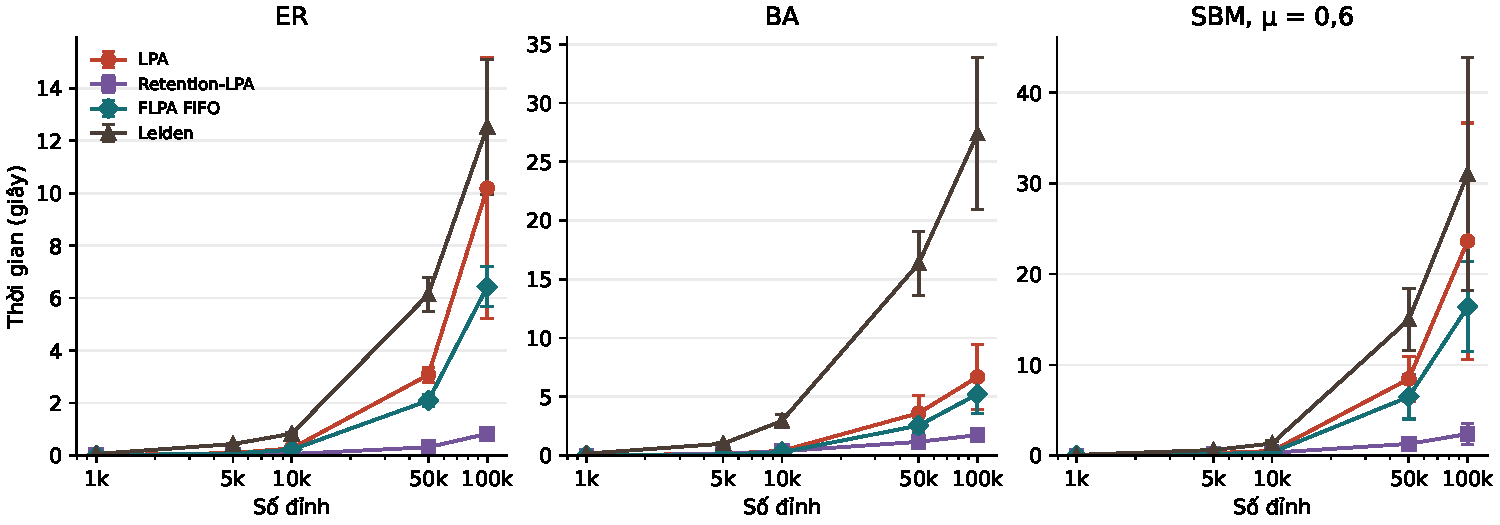
\includegraphics[width=.94\textwidth]{runtime.pdf}
\caption{E1. Thời gian theo kích thước đồ thị. Mỗi điểm là trung bình 10 lượt và vạch sai số là $\pm$ một SD mẫu. Trục số đỉnh theo log để nhìn rõ các kích thước nhỏ.}
\label{fig:e1rt}
\end{figure*}

\begin{figure*}[t]
\centering
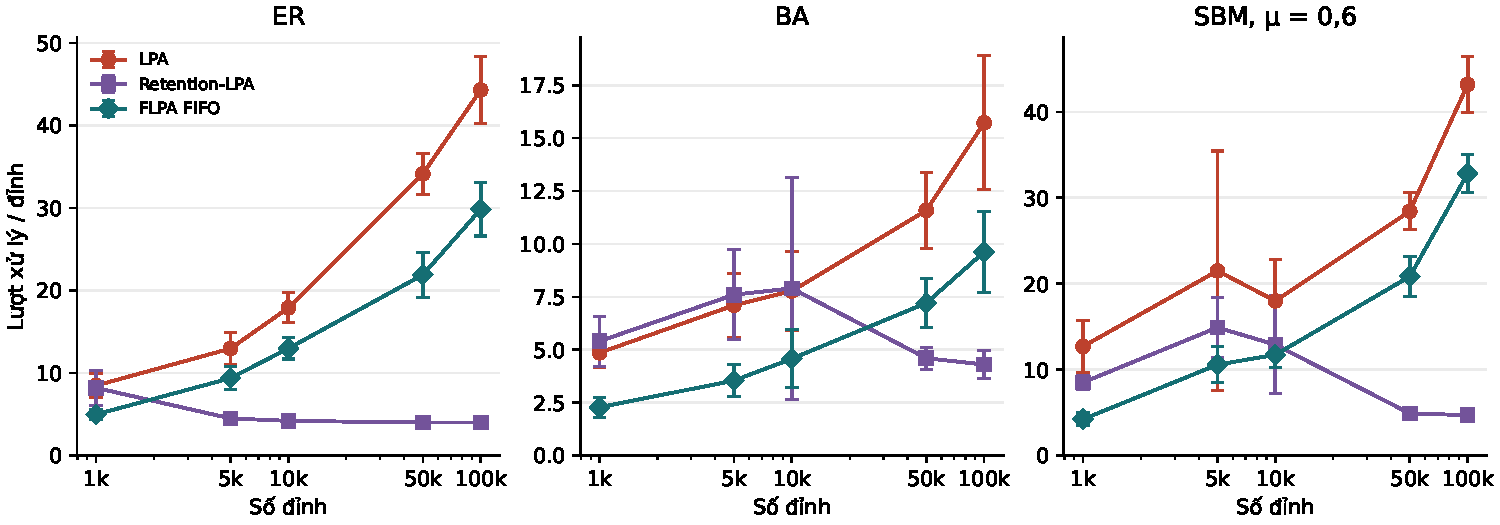
\includegraphics[width=.94\textwidth]{work.pdf}
\caption{E1. Số lượt xử lý trên mỗi đỉnh, kể cả kiểm tra dừng của LPA. Leiden không có bộ đếm này.}
\label{fig:e1work}
\end{figure*}

\begin{table}[t]
\centering
\caption{E1 ở 100.000 đỉnh. Thời gian là mean $\pm$ SD, số lượt và số cụm là mean.}
\label{tab:e1}
\resizebox{\columnwidth}{!}{\EoneTable}
\end{table}

\begin{table}[t]
\centering
\caption{E1 ở 50.000 đỉnh. Điểm Figure 1 xấp xỉ, sai số đọc khoảng 0,05 giây.}
\label{tab:paper}
\resizebox{\columnwidth}{!}{\PaperTable}
\end{table}

\begin{table}[t]
\centering
\caption{Python và mã C tác giả trên cùng đồ thị 100.000 đỉnh và cùng seed số.}
\label{tab:author}
\resizebox{\columnwidth}{!}{\AuthorTable}
\end{table}

E1 hoàn thành 600/600 lượt trên 15 cấu hình. Hình~\ref{fig:e1rt} cho thấy runtime tăng cùng kích thước trong ba họ đồ thị. Hình~\ref{fig:e1work} đối chiếu số lượt xử lý đỉnh. Bảng~\ref{tab:e1} tóm tắt các cấu hình 100.000 đỉnh. LPA và FLPA có cùng bước tính phiếu. Bên cạnh số lượt, phân bố bậc tại các đỉnh được ghé và lần quét để đưa lại láng giềng cũng ảnh hưởng thời gian.

Trên ER 100.000 đỉnh, LPA dùng trung bình 44,30 lượt trên một đỉnh, còn FLPA dùng 29,84. Thời gian trung bình lần lượt là 10,190 và 6,435 giây. Trung bình tỷ lệ ghép cặp LPA/FLPA là $1.58\pm0.69$. Ở mỗi seed, cả hai trả về một cụm lớn cùng một nhãn riêng cho từng đỉnh cô lập. Vì vậy số cụm trung bình 6,3 chủ yếu phản ánh chính sách giữ isolate. Retention-LPA dừng ở trung bình 0,831 giây và trả hơn 31.000 nhóm. Tốc độ của retention đi cùng một nghiệm rất mịn, cũng là xu hướng tác giả quan sát trên ER.

Trên BA 100.000 đỉnh, LPA và FLPA cùng trả một cụm ở cả 10 lần, với thời gian lần lượt $6.679\pm2.780$ và $5.223\pm1.672$ giây. Trung bình tỷ lệ ghép cặp là $1.30\pm0.34$. FLPA giảm lượt đỉnh từ 15,73 xuống 9,62 lượt trên đỉnh. Quét lại láng giềng khi cập nhật hub vẫn có chi phí đáng kể. Retention-LPA tạo khoảng 27.403 cụm trung bình. Leiden thu được trung bình 21,9 cụm và $Q=0.295$. Do BA thiếu nhãn chuẩn, số cụm và modularity cho thấy các dạng phân hoạch khác nhau và làm rõ ảnh hưởng của mục tiêu tối ưu.

SBM 100.000 đỉnh có bậc trung bình thực từ 9,984 đến 10,025 và phần cạnh ngoại khối từ 0,5994 đến 0,6013. Tỷ lệ thời gian LPA/FLPA là $1.40\pm0.54$ theo cặp. LPA và FLPA lần lượt có khoảng 43,18 và 32,83 lượt xử lý trên mỗi đỉnh. Cả hai có NMI xấp xỉ 0 và ACC xấp xỉ 0,01 tại $\mu=0.60$. Retention-LPA cho NMI 0,508 trong khi ARI là 0,0015 và ACC là 0,0059 với hơn 31.000 cụm. Các mảnh nhỏ mang thông tin về nhóm gốc theo NMI, nhưng rất ít cặp cùng nhóm được giữ và các mảnh dư bị phạt khi ghép một-một. Leiden đạt modularity 0,303 trên cấu hình này và NMI 0,021. Hai mục tiêu chất lượng đánh giá những đặc tính khác nhau của phân hoạch.

Bảng~\ref{tab:paper} đưa ra thời gian Figure~1 tại 50.000 đỉnh và độ lệch tương đối của bản Python. Gọi $\bar t_P$ là mean đo được bằng Python và $\bar t_R$ là mean tham chiếu từ hình hoặc phép đo C. Cột sai lệch dùng phần trăm
\begin{equation}
  \Delta = 100\left(\frac{\bar t_P}{\bar t_R}-1\right).
  \label{eq:deviation}
\end{equation}
Điểm tham chiếu từ hình được làm tròn đến 0,05 giây. Độ lệch tương đối dễ nhạy với sai số đọc khi $\bar t_R$ nhỏ. Panel tăng kích thước cắt một số điểm lớn, nên so sánh SBM 100.000 đỉnh tại $\mu=0.60$ sử dụng panel thay đổi $\mu$. Ở panel đó, thời gian LPA và FLPA xấp xỉ 5,80 và 2,70 giây, tỷ số khoảng 2,15. Thử nghiệm Python cho tỷ số của hai mean là 1,44 và mean các tỷ số ghép là 1,40. Cả ba họ đều cho FLPA nhanh hơn LPA theo trung bình ghép cặp ở tất cả kích thước, trong khoảng 1,20–2,46 lần. Độ lớn cải thiện khác nhau theo họ và kích thước. Mốc trên 700 lần trong bài báo thuộc mạng us-patents, được báo cáo ở Bảng~2~\cite{flpa}.

Bảng~\ref{tab:author} bổ sung phép đo trên cùng topology bằng mã C. Cả 54 lượt C hoàn thành ở hai kích thước 10.000 và 100.000. Tại 100.000 đỉnh, tỷ số mean LPA/FLPA của C là 1,98 trên ER, 2,50 trên BA và 2,39 trên SBM. Trên đúng ba cặp seed, thời gian FLPA Python/C có tỷ số mean lần lượt 4,49, 12,93 và 18,06. Ở SBM, FLPA của cả hai backend đều có NMI xấp xỉ 0,0001. Retention-LPA ở cả hai backend trả khoảng 31.000 cụm và có NMI gần 0,509. Hai kết quả này cho thấy hiện tượng gộp cụm và phân mảnh cũng xuất hiện ở mã tham chiếu cùng đồ thị.

Phép so sánh C giữ nguyên cạnh và seed số trên cùng máy Apple M1. Hai backend có thể khác RNG, thứ tự duyệt, cấu trúc lưu trữ và chi phí bộ đếm. Chênh lệch với Figure~1 còn chịu ảnh hưởng của Xeon E5-2697, số lần lặp 10 và 2.000, generator và phiên bản thư viện. Khi đánh giá độ lớn của lợi ích FLPA, cần đọc cả độ lệch chuẩn, số lượt xử lý và kiểu phân hoạch mà mỗi thuật toán tạo ra.


\subsection{E3 — ablation thứ tự và quy tắc đưa lại}
\label{sec:e3}

\begin{figure*}[t]
\centering
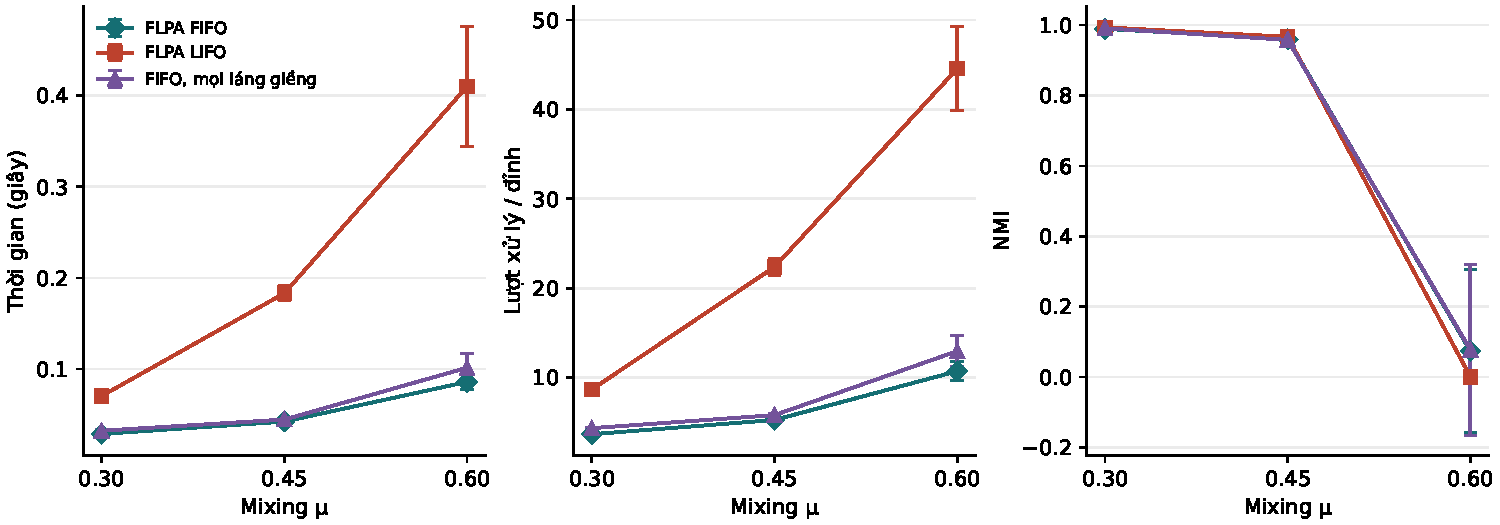
\includegraphics[width=.94\textwidth]{ablation.pdf}
\caption{E3. Chi phí và NMI của ba biến thể FLPA trên SBM 5.000 đỉnh. Điểm là mean và vạch là $\pm$ một SD mẫu trong 10 lần.}
\label{fig:e3}
\end{figure*}

\begin{table*}[t]
\centering
\caption{E3. Chất lượng, công việc và thời gian. Thời gian và các chỉ số có nhãn là mean $\pm$ SD, còn lượt, đổi nhãn và số cụm là mean. Mọi biến thể đều hoàn thành 10/10 cho mỗi $\mu$ và qua kiểm tra maximality.}
\label{tab:e3}
\EthreeTable
\end{table*}

Hình~\ref{fig:e3} và Bảng~\ref{tab:e3} so sánh ba biến thể trên 90 lượt hoàn thành. Thay \texttt{popleft} bằng \texttt{pop} làm lịch xử lý thiên về láng giềng vừa được đưa lại. Cùng một hoán vị ban đầu, LIFO bắt đầu từ đầu còn lại của hàng đợi. Chọn cùng seed và cùng quy tắc phá hoà làm hai biến thể tái lập được trong riêng mỗi lịch, nhưng sau khi thứ tự xử lý khác nhau, thứ tự lấy số ngẫu nhiên cũng khác. Đối chiếu enqueue-all giữ FIFO và cho mọi láng giềng chưa chờ xử lý trở lại hàng đợi sau một cập nhật.

Tại $\mu=0.30$, LIFO xử lý trung bình 43.296 lượt so với 18.293 ở FIFO, đổi nhãn xấp xỉ gấp đôi và tốn thời gian trung bình ghép cặp gấp $2.45\pm0.14$ lần. Chất lượng theo ACC tăng từ 0,966 lên 0,985, với số nhóm trung bình 100,2 sát 100 nhóm thật. Tại $\mu=0.45$, chi phí LIFO tăng lên $4.34\pm0.23$ lần, còn ACC tăng khoảng 0,023 trong khi NMI tăng khoảng 0,006. Cả hai lịch tìm được cấu trúc rõ ở hai mức này. Chất lượng nhích lên có thể có giá trị tùy mục tiêu, nhưng cần cân nhắc số lượt xử lý tăng.

Tại $\mu=0.60$, tỷ lệ thời gian LIFO/FIFO ghép cặp là $4.82\pm0.91$ theo~\eqref{eq:speedup}. LIFO quy về một cụm ở 10/10 lần, với NMI và ARI bằng 0, ACC bằng 0,01. FIFO dự đoán 12,4 cụm trung bình, NMI chỉ 0,073, thể hiện khó khôi phục 100 khối trong cấu hình này. Mỗi biến thể vẫn có maximality 100\% trong các lượt hoàn thành. Một cơ chế phù hợp là LIFO ưu tiên kéo dài quỹ đạo của nhóm đỉnh vừa đổi, dẫn tới bành trướng nhãn trong đồ thị nhiều cạnh giữa nhóm. Ablation đo kết quả và công việc. Kiểm tra cơ chế này sẽ cần trace chi tiết của từng diễn tiến nhãn.

Bỏ điều kiện lọc và đưa lại mọi láng giềng làm số lượt tăng lần lượt khoảng 3.387, 2.706 và 11.234 ở ba mức $\mu$, còn thời gian ghép cặp tăng khoảng 12,4\%, 5,4\% và 18,9\%. Chênh lệch NMI trung bình đều dưới 0,004 theo trị tuyệt đối. Bốc lại nhãn trong thế hoà có thể tạo quỹ đạo mới và đưa thuật toán đến một phân hoạch maximal khác. Kết quả trên ba cấu hình gợi ý rằng lọc chọn láng giềng giảm đánh giá lại, với dao động nhỏ về chất lượng trong mẫu này. E3 chỉ thay một yếu tố mỗi lần trên một họ đồ thị và một kích thước, nên tác động của LIFO lên hub BA hoặc mạng email vẫn cần phép đo riêng.

\subsection{Phần thực nghiệm tích hợp của TV2}
Figure~4 trái của bài báo dùng SBM 100.000 đỉnh và khảo sát NMI theo $\mu$. Bài báo tường thuật giảm độ khôi phục quanh $\mu=0.4$ đến $0.5$~\cite{flpa}. E3 hiện tại dùng 5.000 đỉnh và được thiết kế để đánh giá variant hàng đợi. E2 của TV2 cần đo đủ sweep Figure~4, còn E4 cần đánh giá trên mạng email-Eu-core với nhãn phòng ban. Các bảng và kết luận nhóm về E2/E4 phụ thuộc vào kết quả thực nghiệm từ TV2.
